\chapter{Results}
\label{sec:results}

% Part 1: descriptive mapping (this file, drafted 18 July 2026).
% Part 2: analytical synthesis of conditions — next writing step.
% All numbers below are derived from corpus/coding_table.csv (n = 67, all rows final);
% figures generated by corpus/make_figures.py.

This chapter reports the evidence in two steps. Section~\ref{sec:results-mapping} maps the 67 included studies descriptively: where the evidence comes from and how it is produced. Section~\ref{sec:results-synthesis} then synthesizes the conditions under which firm-level AI investments translate into performance gains or competitive advantage. All counts, groupings, and figures in this chapter are the author's own compilation from the coding table; the full table is reported in the appendix.

\section{Descriptive mapping of the evidence base}
\label{sec:results-mapping}

The search window ran from 2015 to 2026, yet the earliest included study dates from 2020 (Figure~\ref{fig:year}). Growth is concentrated at the end of that window: 44 of the 67 studies, two thirds of the corpus, appeared in 2025 and 2026 alone. The evidence base is young.

\begin{figure}[htbp]
  \centering
  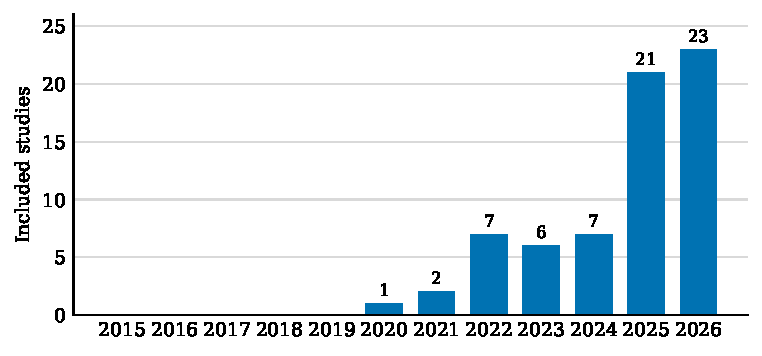
\includegraphics[width=\textwidth]{figures/fig_year}
  \caption{Included studies per publication year, search window 2015--2026 (n = 67). Source: own representation based on the coding table.}
  \label{fig:year}
\end{figure}

The 67 studies are spread across 45 journals, with no dominant outlet: Industrial Marketing Management and the Journal of Business Research lead with five studies each, followed by Technology in Society, the International Review of Financial Analysis, and the International Journal of Information Management with four each. Journal quality within the corpus is skewed toward the middle of the AJG scale (Figure~\ref{fig:ajg}): 27 studies come from journals rated 2, another 33 from journals rated 3, and seven from journals rated 4 or 4*.

\begin{figure}[htbp]
  \centering
  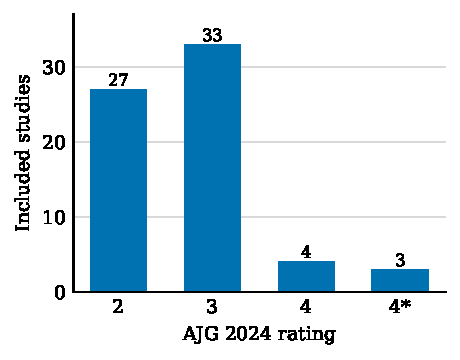
\includegraphics[width=0.55\textwidth]{figures/fig_ajg}
  \caption{Included studies by AJG 2024 journal rating (n = 67). Source: own representation based on the coding table.}
  \label{fig:ajg}
\end{figure}

Two research designs dominate the corpus (Figure~\ref{fig:method}): panel econometrics on archival firm data (27 studies) and survey-based structural equation modeling (24 studies). The remaining sixteen studies combine several methods (six), examine stock market reactions in event studies (four), or build on case evidence (three); fsQCA, data envelopment analysis, and survey-based regression appear once each. The way studies operationalize AI investment splits the corpus in half: 33 studies rely on managers' self-reports through survey constructs, 31 on archival measures, and three on qualitative observation. Disclosure text mining (seven studies), patent-based proxies (six), workforce-based measures such as AI job postings (five), and investment announcements (four) account for most of the archival measures; the remaining nine rest on single-study instruments, for example procurement records or exposure to an AI policy shock.

\begin{figure}[htbp]
  \centering
  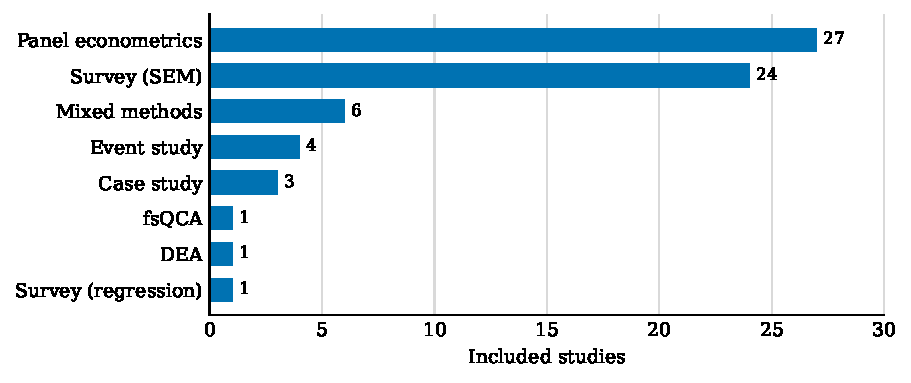
\includegraphics[width=\textwidth]{figures/fig_method}
  \caption{Included studies by research design (n = 67). Source: own representation based on the coding table.}
  \label{fig:method}
\end{figure}

Study samples cluster in two countries (Figure~\ref{fig:geography}): the USA and China account for 16 studies each, together almost half of the corpus. India follows with seven studies, and another seven draw on multi-country samples. European firms appear in ten studies: four multi-country European samples plus six single-country ones. Most samples span several industries: 39 studies are cross-industry, ten focus on manufacturing, and the rest examine single settings such as healthcare or high-tech ventures.

\begin{figure}[htbp]
  \centering
  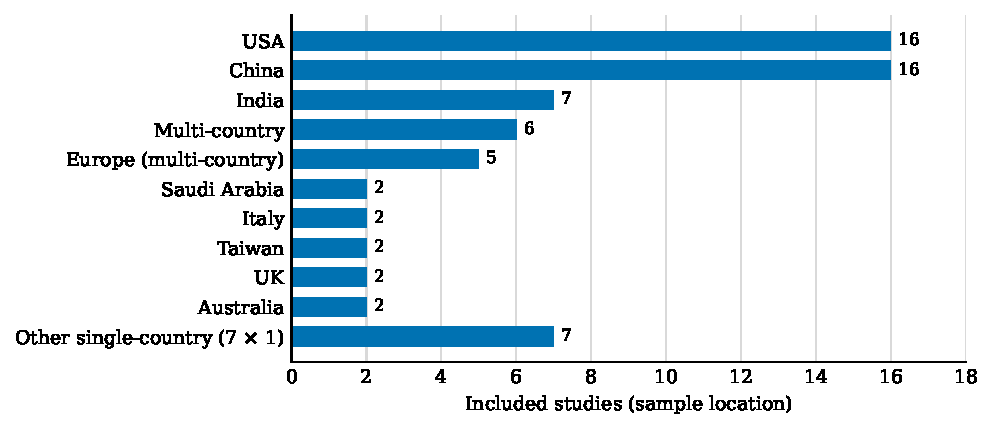
\includegraphics[width=\textwidth]{figures/fig_geography}
  \caption{Included studies by sample location (n = 67). Source: own representation based on the coding table.}
  \label{fig:geography}
\end{figure}

Following the distinction between superior firm performance and competitive advantage introduced in Chapter~\ref{sec:background}, the coding recorded which of the two constructs each study measures (Figure~\ref{fig:outcome}). The result is one-sided: 52 of the 67 studies measure firm performance only. Six measure competitive advantage as a distinct construct, and nine measure both. Measured competitive advantage is thus rare in this literature: 15 studies, under a quarter of the corpus. Effect directions spread across all four codes: 38 studies report a positive average effect of AI investment on their outcome, 20 an effect that exists only through a mechanism or under specific circumstances, five results that split across outcome indicators, and four negative effects. Among the 15 studies with a competitive-advantage construct, ten find positive and five conditional effects; none reports a negative one.

\begin{figure}[htbp]
  \centering
  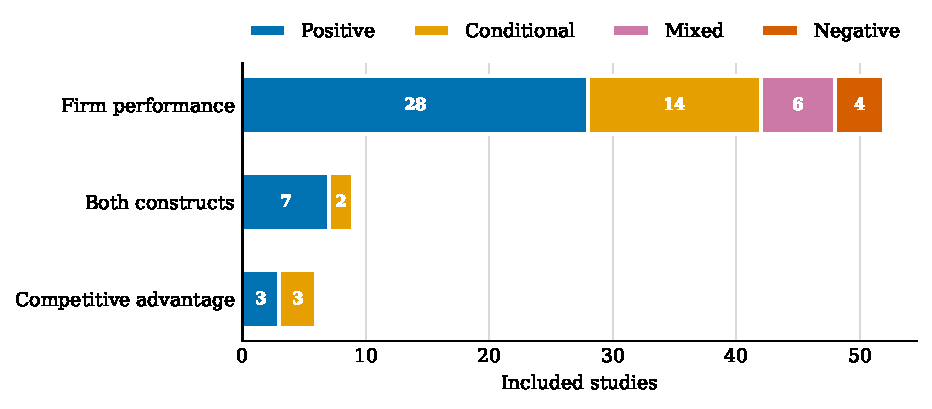
\includegraphics[width=\textwidth]{figures/fig_outcome_direction}
  \caption{Outcome construct by reported effect direction (n = 67). Source: own representation based on the coding table.}
  \label{fig:outcome}
\end{figure}

Conditions are the rule, not the exception: 63 of the 67 studies identify at least one moderator, mediator, complement, or threshold that shapes the link between AI investment and its outcome. Only four studies report unconditional evidence. Section~\ref{sec:results-synthesis} orders these conditions.

\section{Synthesis of conditions}
\label{sec:results-synthesis}

% Part 2 — analytical synthesis of the identified conditions (next writing step).
